\documentclass[a4paper]{article}
\usepackage{graphicx}
\usepackage[absolute,overlay]{textpos}
\usepackage{background}
\usepackage{times}
\usepackage{lmodern}
\usepackage{geometry}
\geometry{a4paper,left=1.5cm,right=1cm,top=1cm,bottom=1cm,columnsep=0.8cm}
\usepackage{fontawesome5}
\usepackage[hidelinks]{hyperref}
\usepackage{fontspec}
\setmainfont{Arial}
\usepackage{eso-pic}

\definecolor{texcolor}{HTML}{e2e8f0}
%Ne touchez pas cette image c'est mon background tu laisse le nom comme ça.

\AddToShipoutPictureBG*{ 
  
\includegraphics[width=\paperwidth,height=\paperheight]{background.jpg}
}

\newcommand{\cvsection}[1]{
\begin{tabular}{@{}p{0.26\linewidth}}
\\
\textbf{\Large #1}  \\[10pt]
\end{tabular}
}

\newcommand{\cicon}{\tikz[baseline]{\draw[fill=white] (0,0.1) circle [radius=0.25cm];}~ }

\setlength{\parindent}{0pt}

\begin{document}


%% Change le nom photo.jpg par le nom de la photo que tu as reçu.
\begin{textblock*}{4cm}(0.2cm,0.3cm) % largeur x (x, y) depuis le coin haut gauche
  \includegraphics[width=2.5cm,clip,keepaspectratio]{photo.jpg}
\end{textblock*}




\color{texcolor}

\begin{center}
{\fontsize{44pt}{24pt}\selectfont \textbf{name}}

~

{\Large Titre}

~

~

\faMapMarker ~ {address}  ~ ~ \faEnvelope  ~ \href{mailto:email}{{email}}

~

\begin{tikzpicture}
  \node[draw, fill=white, rounded corners=9pt, inner xsep=8pt, inner ysep=4pt, align=center] 
    {\color{black}\faGlobe~\href{website}{website}};
\end{tikzpicture}
~ ~ 
\begin{tikzpicture}
  \node[draw, fill=white, rounded corners=9pt, inner xsep=8pt, inner ysep=4pt, align=center] 
    {\color{black}\faFigma~\href{website}{website}};
\end{tikzpicture}
~ ~ 
\begin{tikzpicture}
  \node[draw, fill=white, rounded corners=9pt, inner xsep=8pt, inner ysep=4pt, align=center] 
    {\color{black}\faGithub~\href{GitHub}{website}};
\end{tikzpicture}
\end{center}

\vspace{-0.3cm}

\hspace{-1.5cm}\rule{\paperwidth}{0.4pt}


\begin{tabular}{@{}p{0.26\linewidth}p{0.7\linewidth}}
\\
\textbf{\Large Profil} 
%% Profil %%

\end{tabular}

~

\rule{\linewidth}{0.05pt}


\begin{tabular}{@{}p{0.26\linewidth}p{0.7\linewidth}}
\\
\textbf{\Large Education} & 
{education[0].degree} \hfill {\small{education[0].start}-{education[0].end}} \\
& {education[0].institution} \\

{education[1].degree} \hfill {\small{education[1].start}-{education[1].end}} \\
& {education[1].institution} \\

\end{tabular}

~

\rule{\linewidth}{0.05pt}

\begin{tabular}{@{}p{0.26\linewidth}p{0.7\linewidth}}
\\
\textbf{\Large Experience} & 
\textbf{{experience[0].title}} \hfill {\small{experience[0].start}-{experience[0].end}} \\[6pt]
& \textbf{{experience[0].company}} \\[6pt]
& {experience[0].description[0]} \\[6pt]
& {experience[0].description[1]} \\[6pt]
& {experience[0].description[2]} \\
\end{tabular}

~

\rule{\linewidth}{0.05pt}

\begin{tabular}{@{}p{0.26\linewidth}p{0.18\linewidth}p{0.18\linewidth}p{0.18\linewidth}}
\\
\textbf{\Large Skills} & 
\cicon {skills[1]} & \cicon {skills[2]} & \cicon {skills[3]} \\[6pt]
& 
\cicon {skills[4]} & \cicon {skills[5]} & \cicon {skills[6]} \\[6pt]
& 
\cicon {skills[7]} & \cicon {skills[8]} & \cicon {skills[9]} \\[6pt]
& 
\cicon {skills[10]} & \cicon {skills[11]} & \cicon {skills[12]} \\
\end{tabular}



\end{document}
